
\subsection{EL}\label{el}

Ein EL-Konzept ist ein ALC-Konzept, in dem nur die Konstruktoren
$\top,\ $ $\sqcap$ und $\exists r.C$ verwendet werden.

\subsection{Simulation}\label{simulation}

Simulation ist gerichtete Bisimulation.
$\left( I_{1},d_{1} \right) \precsim \left( I_{2},d_{2} \right)$: es
gibt Simulation $p$ von $I_{1}$ nach $I_{2}$ mit
$d_{1}\text{\ p\ }d_{2}$.

\hypertarget{lemma-6.3}{\subsubsection{Lemma 6.3}\label{lemma-6.3}}

Seien $I_{1},I_{2}$ Interpretationen, $d_{1} \in \Delta^{I_{1}}$ und
$d_{2} \in \Delta^{I_{2}}$. Wenn
$\left( I_{1},d_{1} \right) \precsim \left( I_{2},d_{2} \right)$, dann
gilt für alle EL-Konzepte $C$: $d_{1} \in C^{I_{1}}$ impliziert
$d_{2} \in C^{I_{2}}$.

Beweisskizze per Induktion über die Struktur von $C$. Sei $\rho$
eine Simulation zwischen $I_{1}$ und $I_{2}$ mit
$d_{1}\text{\ $\rho$}\text{\ d}_{2}$.

\textbf{I.A.} $C = A$ ist Konzeptname. Nach Bedingung 1. der
Bisimulation gilt $d_{1} \in A^{I_{1}}$ impliziert
$d_{2} \in A^{I_{2}}$.

\textbf{I.S.} Unterscheide Fälle gemäß dem äußersten Konstrukt von
$C$.

\begin{enumerate}
\def\labelenumi{\arabic{enumi}.}
\item
  $C = D_{1} \sqcap D_{2}$
\end{enumerate}

\begin{quote}
$d_{1} \in C^{I_{1}}$ gdw. $d_{1} \in D_{1}^{I_{1}}$und
$d_{1} \in D_{2}^{I_{1}}$ (Semantik) impliziert.
$d_{2} \in D_{1}^{I_{2}}$ und $d_{2} \in D_{2}^{I_{2}}$ (I.V.) gdw.
$d_{2} \in C^{I_{2}}$ (Semantik)
\end{quote}

\begin{enumerate}
\def\labelenumi{\arabic{enumi}.}
\item
  $C = \exists r.D$
\end{enumerate}

\begin{quote}
Hinrichtung und Rückrichtung analog über Semantik, 2. Bedingung der
Simulation, I.V., Semantik.
\end{quote}

\subsubsection{Lemma 6.4}\label{lemma-6.4}

Bisimulation und wechselseitige Simulation sind nicht dasselbe.

Beweisskizze: Zeige Wechselseitige Simulation, die keine Biosimulation
ist:

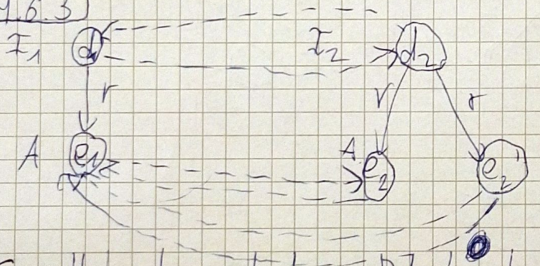
\includegraphics[width=3.71910in,height=1.83200in]{media/image1.png}

\subsubsection{Lemma 6.6}\label{lemma-6.6}

Jedes EL-Konzept ist erfüllbar bzgl. jeder TBox.

Beweisskizze per Induktion über die Struktur von $C$:

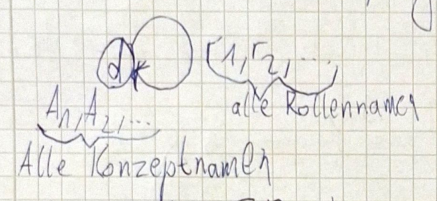
\includegraphics[width=2.50460in,height=1.15200in]{media/image2.png}

\subsection{Subsumtion ohne TBox}\label{subsumtion-ohne-tbox}

Eine Subsumption $C \sqsubseteq D$ gilt in EL im Prinzip gdw mann
$D$ syntaktisch in $C$ „wiederfindet``. Werden Konzepte als
Baummodell dargestellt entspricht „Wiederfinden`` Simulation von
$D$-Baum in $C$-Baum (also Teilgraphenproblem).

\subsubsection{Definition kanonisches
Modell}\label{definition-kanonisches-modell}

Baue aus dem gegebenen Konzept $C$ intuitiv Baummodell.

\hypertarget{lemma-6.8}{\subsubsection{Lemma 6.8}\label{lemma-6.8}}

Für alle EL-Konzepte $C$ gilt: Die Interpretation $I_{C}$ ist Modell
von $C$ mit $d_{w} \in C^{I_{C}}$.

Beweisskizze per Induktion über die Struktur von $C$.

\hypertarget{lemma-6.9}{\subsubsection{Lemma 6.9}\label{lemma-6.9}}

Für alle EL-Konzepte $C$, Interpretation $I$ und
$e \in \Delta^{I}$ gilt: $e \in C^{I}$ gdw.
$\left( I_{C},d_{w} \right) \precsim \left( I,e \right)$.

Beweisskizze.

\begin{itemize}
\item
  Hinrichtung per Induktion über $C$. Schau jeweils Simulation nach
  I.V. an und ergänze diese.
\item
  Rückrichtung. Angenommen
  $\left( I_{C},d_{w} \right) \precsim \left( I,e \right)$.
  \protect\hyperlink{lemma-6.8}{Lemma 6.8} liefert
  $d_{w} \in C^{I_{C}}$. Nach \protect\hyperlink{lemma-6.3}{Theorem
  6.3} ist $e \in C^{I}$.
\end{itemize}

\subsubsection{Lemma 6.10}\label{lemma-6.10}

Für alle EL-Konzepte $C$, $D$ gilt: $C \sqsubseteq D$ gdw.
$\left( I_{D},d_{w} \right) \precsim \left( I_{C},d_{w} \right)$

Beweisskizze.

\begin{itemize}
\item
  Hinrichtung: Betrachte kanonisches Modell $I_{C}$ von $C$. Wegen
  Lemma 6.8 gibt es $d_{w} \in C^{I_{C}}$. Mit $C \sqsubseteq D$
  folgt $d_{W} \in D^{I_{C}}$. Mit \protect\hyperlink{lemma-6.9}{Lemma
  6.9} folgt für $D,\ I_{C},d$ dass $d_{w} \in D^{I_{C}}$ gdw.
  $\left( I_{D},d_{w} \right) \precsim \left( I_{C},d_{w} \right)$.
\item
  Rückrichtung. Angenommen
  $\left( I_{D},d_{w} \right) \precsim \left( I_{C},d_{w} \right)$.
  Betrachte beliebige Interpretation $I$ und $d \in C^{I}$. Zu
  zeigen: $d \in D^{I}$. Wegen $d \in C^{I}$ und
  \protect\hyperlink{lemma-6.9}{Lemma 6.9} gilt
  $\left( I_{C},d_{w} \right) \precsim \left( I,d \right)$. Verkette
  die Simulationen so dass
  $\left( I_{D},d_{w} \right) \precsim \left( I,d \right)$. Mit
  \protect\hyperlink{lemma-6.9}{Lemma 6.9} folgt
  $d_{w} \in D^{I_{C}}$.
\end{itemize}

\subsubsection{Theorem 6.11}\label{theorem-6.11}

Subsumtion in EL kann in polynomieller Zeit entschieden werden:

\begin{itemize}
\item
  Konstruiere $I_{C}$ und $I_{D}$ in polynomieller Zeit.
\item
  Überprüfe in polynomieller Zeit, ob
  $\left( I_{D},d_{w} \right) \precsim \left( I_{C},d_{w} \right)$

  \begin{itemize}
  \item
    Berechne maximale Simulation $\varsigma$
  \item
    Teste ob $\left( d_{w},d_{W} \right) \in \varsigma$
  \end{itemize}
\end{itemize}

\subsection{Subsumption mit TBox}\label{subsumption-mit-tbox}

\subsubsection{Lemma 6.12}\label{lemma-6.12}

Seien $C,D$ zwei beliebige $\text{EL}$-Konzepte und $T$ eine
EL-TBox. Sei weiterhin
$T^{'} = T \cup \left\{ A_{C} \sqsubseteq C,D \sqsubseteq A_{D} \right\}$.
mit Konzeptnamen $A_{C},A_{D}$, die nicht in $C,D,T$ vorkommen. Dann
gilt; $T \vDash C \sqsubseteq D$ gdw
$T^{'} \vDash A_{C} \sqsubseteq A_{D}$.

\subsubsection{ Normalform}\label{normalform}

Eine TBox ist in \emph{Normalform}, wenn sie nur Inklusionen folgender
Form enthält:

$A_{1} \sqcap \ldots \sqcap A_{n} \sqsubseteq A$
$A \sqsubseteq \exists r.A_{1}$ $\exists r.A \sqsubseteq A_{1}$

\subsubsection{Lemma 6.14}\label{lemma-6.14}

Jede EL-TBox $T$ kann in polynomieller Zeit in eine TBox $T^{'}$ in
Normalform gewandelt werden, so dass für alle Konzeptnamen $A,B$ in
$T$ gilt: $T \vDash A \sqsubseteq B$ gdw
$T \vDash A \sqsubseteq B$. Dann ist $T'$ \emph{konservative
Erweiterung} von $T$.

\subsubsection{Lemma 6.14}\label{lemma-6.14-1}

Jede EL-TBox $T$ kann durch linear viele Regelanwendungen in TBox in
Normalform transformiert werden, die konservative Erweiterung von $T$
ist.

Die Regeln fügen jeweils Zwischenkonzepte ein.

Beweisskizze: Grad der Abnormalität definieren und zeigen, dass

\begin{enumerate}
\def\labelenumi{\arabic{enumi}.}
\item
  Der Grad ist beschränkt durch $\left| T \right|$
\item
  Jede Regelanwendung verringert den Grad
\item
  TBoxen vom Grad $0$ sind in Normalform
\end{enumerate}

\subsubsection{Algorithmus}\label{algorithmus}

Wende Regeln erschöpfend an um alle Subsumptionen zu berechnen:

$\frac{\ }{A \sqsubseteq A}$ (Wenn $A$ in $T$ vorkommt)
$\frac{\ }{A \sqsubseteq \top}$ (Wenn $A$ in $T$ vorkommt)

$\frac{A \sqsubseteq A_{1},\ldots,A \sqsubseteq A_{n},A_{1} \sqcap \ldots \sqcap A_{n} \sqsubseteq B}{A \sqsubseteq B}$
$\frac{A \sqsubseteq \exists r.A_{1},\ A_{1} \sqsubseteq B_{1},\exists r.B_{1} \sqsubseteq B}{A \sqsubseteq B}$

\textbf{Wo gehört das x hin Vorlesung 17?}

Für eine EL-TBox $T$ sei $T*$ das Ergebnis erschöpfender
Regelanwendungen, die \emph{Saturierung}.

\subsubsection{Theorem 6.16 }\label{theorem-6.16}

Für alle Konzeptnamen $A,B$ in $T$ gilt:
$T \vDash A \sqsubseteq B$ gdw $A \sqsubseteq B \in T*$

\paragraph{Terminierung}\label{terminierung-1}

Beweisskizze. Jede Regelanwendung erzeugt eine neue Konzeptinklusion
$A \sqsubseteq B$, wobei $A,B$ Konzeptnamen aus $T$. Es gibt nur
endlich viele solcher Inklusionen.

\paragraph{Korrektheit}\label{korrektheit-1}

Beweisskizze. Sei $T = T_{0},\ \ldots,(T_{n} = T*)$ die durch
Regelanwendungen erzeugte Folge von TBoxen. Es genügt zu zeigen:
$T_{i} \vDash T_{i + 1}$. Zeige dies durch Vorbedingung der
Regelanwendung und der Semantik.

\paragraph{Vollständigkeit}\label{vollstuxe4ndigkeit-1}

\subparagraph{Kanonische
Interpretation}\label{kanonische-interpretation}

Die Kanonische Interpretation $I$ ist:

\begin{itemize}
\item
  $\Delta^{I} = \left\{ d_{A}\ |\ A\ \mathrm{\text{Konzeptname\ in\ T}}* \right\} \cup \left\{ d_{\top} \right\}$
\item
  $A^{I} = \left\{ d_{\text{B\ }} \middle| \ B \sqsubseteq A \in T* \right\}$
\item
  $r^{I} = \left\{ \left( d_{A},d_{B} \right)\  \middle| \ A \sqsubseteq A^{'} \in T*\ \mathrm{\text{und}}\ A^{'} \sqsubseteq \exists r.B \in T*,\ A^{'}\ \mathrm{\text{Konzeptname}} \right\}$
\end{itemize}

Erklärung: Konstruiere Intuitiv Modell aus allen Konzeptnamen.

\hypertarget{lemma-6.18}{\subparagraph{Lemma 6.18}\label{lemma-6.18}}

Die kanonische Interpretation ist ein Model von $T*$.

Beweis: Zeige, dass alle Inklusionen in $T*$ von $I$ erfüllt werden.
Verwende die Inklusionen in Normalform. Überlege dazu, was aus den
Inklusionen mithilfe der Definition gefolgert werden kann.

\subparagraph{Vollständigkeit}\label{vollstuxe4ndigkeit-2}

Angenommen $A \sqsubseteq B \notin T*$. Betrachte Element $d_{A}$
der kanonischen Interpretation $I$. Wegen R1:
$A \sqsubseteq A \in T*$, also nach Def. $I$: $d_{A} \in A^{I}$.
Def. von $I$ und $A \sqsubseteq B \notin T*$ liefern
$d_{A} \notin B$. Da $I$ Modell von $T*$
(\protect\hyperlink{lemma-6.18}{Lemma 6.18}), und damit von $T$, folgt
nicht $T \vDash A \sqsubseteq B$.

\subsection{Erweiterungen von EL}\label{erweiterungen-von-el}

\hypertarget{el-mit-disjunktion-und-bottom}{\subsubsection{EL mit
Disjunktion und Bottom}\label{el-mit-disjunktion-und-bottom}}

Erfüllbarkeit in $\text{ELU}_{\bot}$ (mit Disjunktion) ist
ExpTime-Vollständig.

Beweisskizze per Reduktion von Erfüllbarkeit von Konzeptname $A$ bzgl.
ALC-TBox $T$:

\begin{enumerate}
\def\labelenumi{\arabic{enumi}.}
\item
  Ersetze Werterestriktion in $T$ durch Existenzrestriktion.
\item
  Bringe $T$ in Negationsnormalform.
\item
  Ersetze $\neg X$ durch $\overset{\overline{}}{X}$ mit
  $\top \sqsubseteq X \sqcup \overset{\overline{}}{X}$ und
  $X \sqcap \overset{\overline{}}{X} \sqsubseteq \bot$
\end{enumerate}

\subsubsection{ELU (mit Disjunktion)}\label{elu-mit-disjunktion}

Erfüllbarkeit in ELU ist ExpTime-Vollständig.

Beweisskizze per Reduktion von
\protect\hyperlink{el-mit-disjunktion-und-bottom}{6.5.1}. Ersetzte
$\bot$ durch $L$ mit $\exists r.L \sqsubseteq L$ für alle
Rollennamen $r$ in $T$.
